\documentclass{beamer}
\usetheme{metropolis}
\usepackage{graphicx}
\usepackage{amsmath}
\usepackage{tcolorbox}
\title{College Writing Seminar (INTD100): Week 2 Notes}
\author{Jordan Hanson}
\institute{Whittier College Department of Physics and Astronomy}

\begin{document}
\maketitle

\section{Summary}

\begin{frame}{Summary}
\textbf{Week 2}: \textit{Concise writing II:} In Week 2, we will focus on reading a piece of science writing, and creating your \textit{own} writing that tailors the story to a particular audience.
\begin{itemize}
\item Exercises: work in teams to produce a piece of science writing intended for a broad audience that weaves together information from a variety of sources: (a) a TED talk (b) a scientific journal article (c) and resources like Wikipedia and Google Scholar
\item Homework: writing a post designed for social media about a piece of science that grabs the attention of a wide audience, and attempts to convince that audience that the science is interesting
\item Exploration topic: Black hole observations
\end{itemize}
\end{frame}

\section{Group Project}

\begin{frame}{Group Project: Collaborative Science Writing}
\textbf{\alert{Instructions}}: Systematically random groups (next slide)
\begin{enumerate}
\item Choose one of the following four topics on the following slides
\item Choose a \textit{corresponding author} who will create a Google Document and share it with the others
\item Select a number of sources pertaining to the topic
\begin{itemize}
\item TED talks
\item Scientific journals from \url{arXiv.org} and \url{scholar.google.com}
\item Sources located on Wikipedia
\end{itemize}
\item Create a map or outline with Coggle.it or other tool that summarizes recent discoveries
\item Write a 1 page, single-spaced, 12 point font summary ($\approx 800-1000$ words)'
\item \alert{Bonus points: including a separate bibliography, correctly formatted}
\end{enumerate}
\end{frame}

\begin{frame}{Group Project: Collaborative Science Writing}
\small
\begin{columns}[T]
\begin{column}{0.5\textwidth}
\begin{enumerate}
\item Grace	Cooper ... Group A
\item Zack	Duhala ... Group B
\item Juan	Estrada ... Group C
\item Jusraunaq	Farmahan ... Group D
\item Mateo	Gomez ... Group A
\item Elise	Hansen ... Group B
\item Wyatt	Killien ... Group C
\item Kyle	Miller ... Group D
\end{enumerate}
\end{column}
\begin{column}{0.5\textwidth}
\begin{enumerate}
\item Eliot	Moser ... Group A
\item Rudy	Reyes ... Group B
\item Nick	Reynolds ... Group C
\item Paulina Valdez ... Group D
\item Andrea Wainwright ... Group A
\item Natasha Waldorf ... Group B
\item Emma Walston ... Group C
\end{enumerate}
\end{column}
\end{columns}
\end{frame}

\begin{frame}{Group Project: Collaborative Science Writing}
\small
\underline{Science Topics}
\begin{enumerate}
\item Event Horizon Telescope and the First Picture of a Black Hole
\begin{itemize}
\item What is long-baseline interferometry?
\item What are the properties of the black hole observed?
\end{itemize}
\item LIGO, Virgo and the First Neutron Star - Black Hole Merger
\begin{itemize}
\item What is a neutron star?
\item What is a black hole neutron stare merger?
\end{itemize}
\item IceCube Neutrino Observatory
\begin{itemize}
\item What is a neutrino?
\item What is IceCube Neutrino Observatory and where is it located?
\item What major discoveries have they made so far?
\end{itemize}
\item Anything related to COVID-19 and the pandemic
\begin{itemize}
\item How is the rate of spread quantified?
\item How fatal is the virus, and how does this vary for people?
\end{itemize}
\end{enumerate}
\end{frame}

\begin{frame}{Group Project: Collaborative Science Writing}
\small
\underline{Source classes}
\begin{enumerate}
\item TED talks: surprisingly useful at the start: \url{https://www.ted.com/talks/katie_bouman_how_to_take_a_picture_of_a_black_hole?utm_campaign=tedspread&utm_medium=referral&utm_source=tedcomshare}
\item Wikipedia has more sources: Event Horizon Telescope \url{https://en.wikipedia.org/wiki/Event_Horizon_Telescope}, references section leads you to \url{arXiv.org} with the exact set of references to journals
\item \url{arXiv.org} and \url{scholar.google.com}, as previously discussed, leads to journals
\item NewScientist, Space.com, Scientific American, etc.
\end{enumerate}
\end{frame}

\begin{frame}{Group Project: Collaborative Science Writing}
\begin{figure}
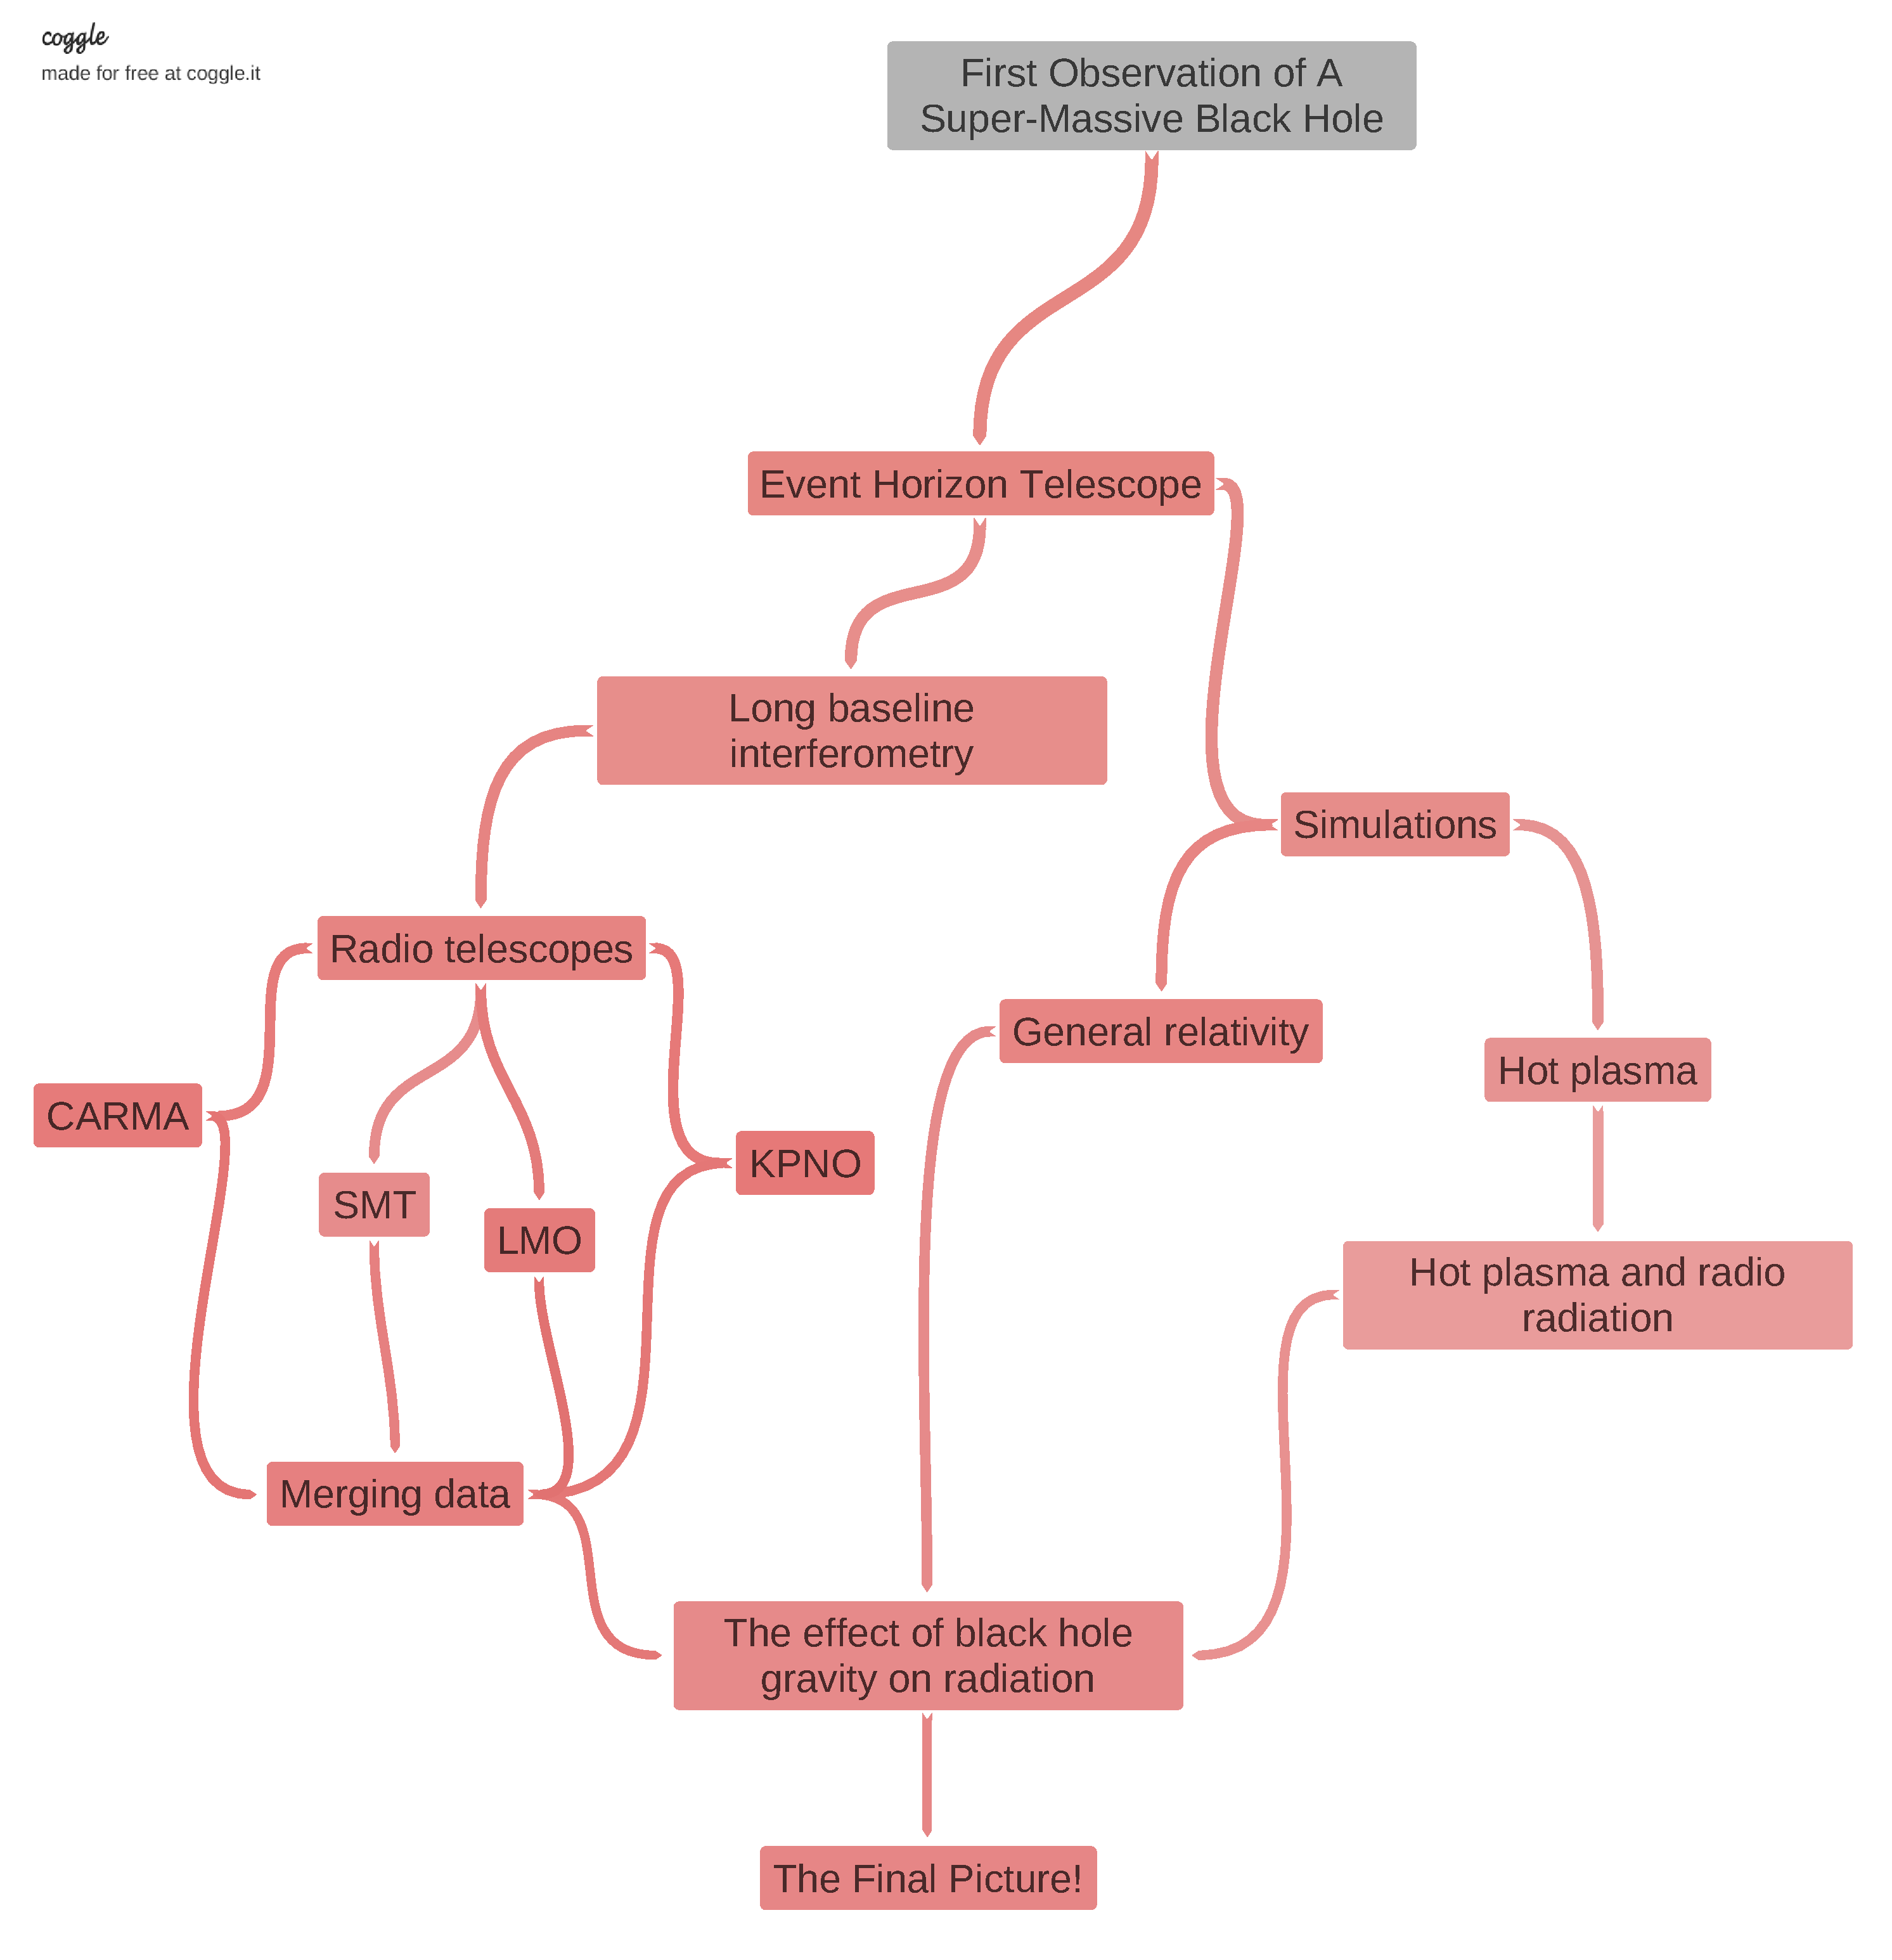
\includegraphics[width=0.65\textwidth]{figures/blackhole.pdf}
\caption{\label{fig:black} Black hole observations and Event Horizon Telescope.}
\end{figure}
\end{frame}

\begin{frame}{Group Project: Collaborative Science Writing}
\underline{Sources to Outline: Which details to cut?}
\begin{enumerate}
\item Kill your darlings
\item Hierarchy of detail: which \textit{level} of detail to cut?
\item Using analogies to replace finest details, equations
\item Cite or quote experts where appropriate
\end{enumerate}
\end{frame}

\begin{frame}{Group Project: Collaborative Science Writing}
\begin{figure}
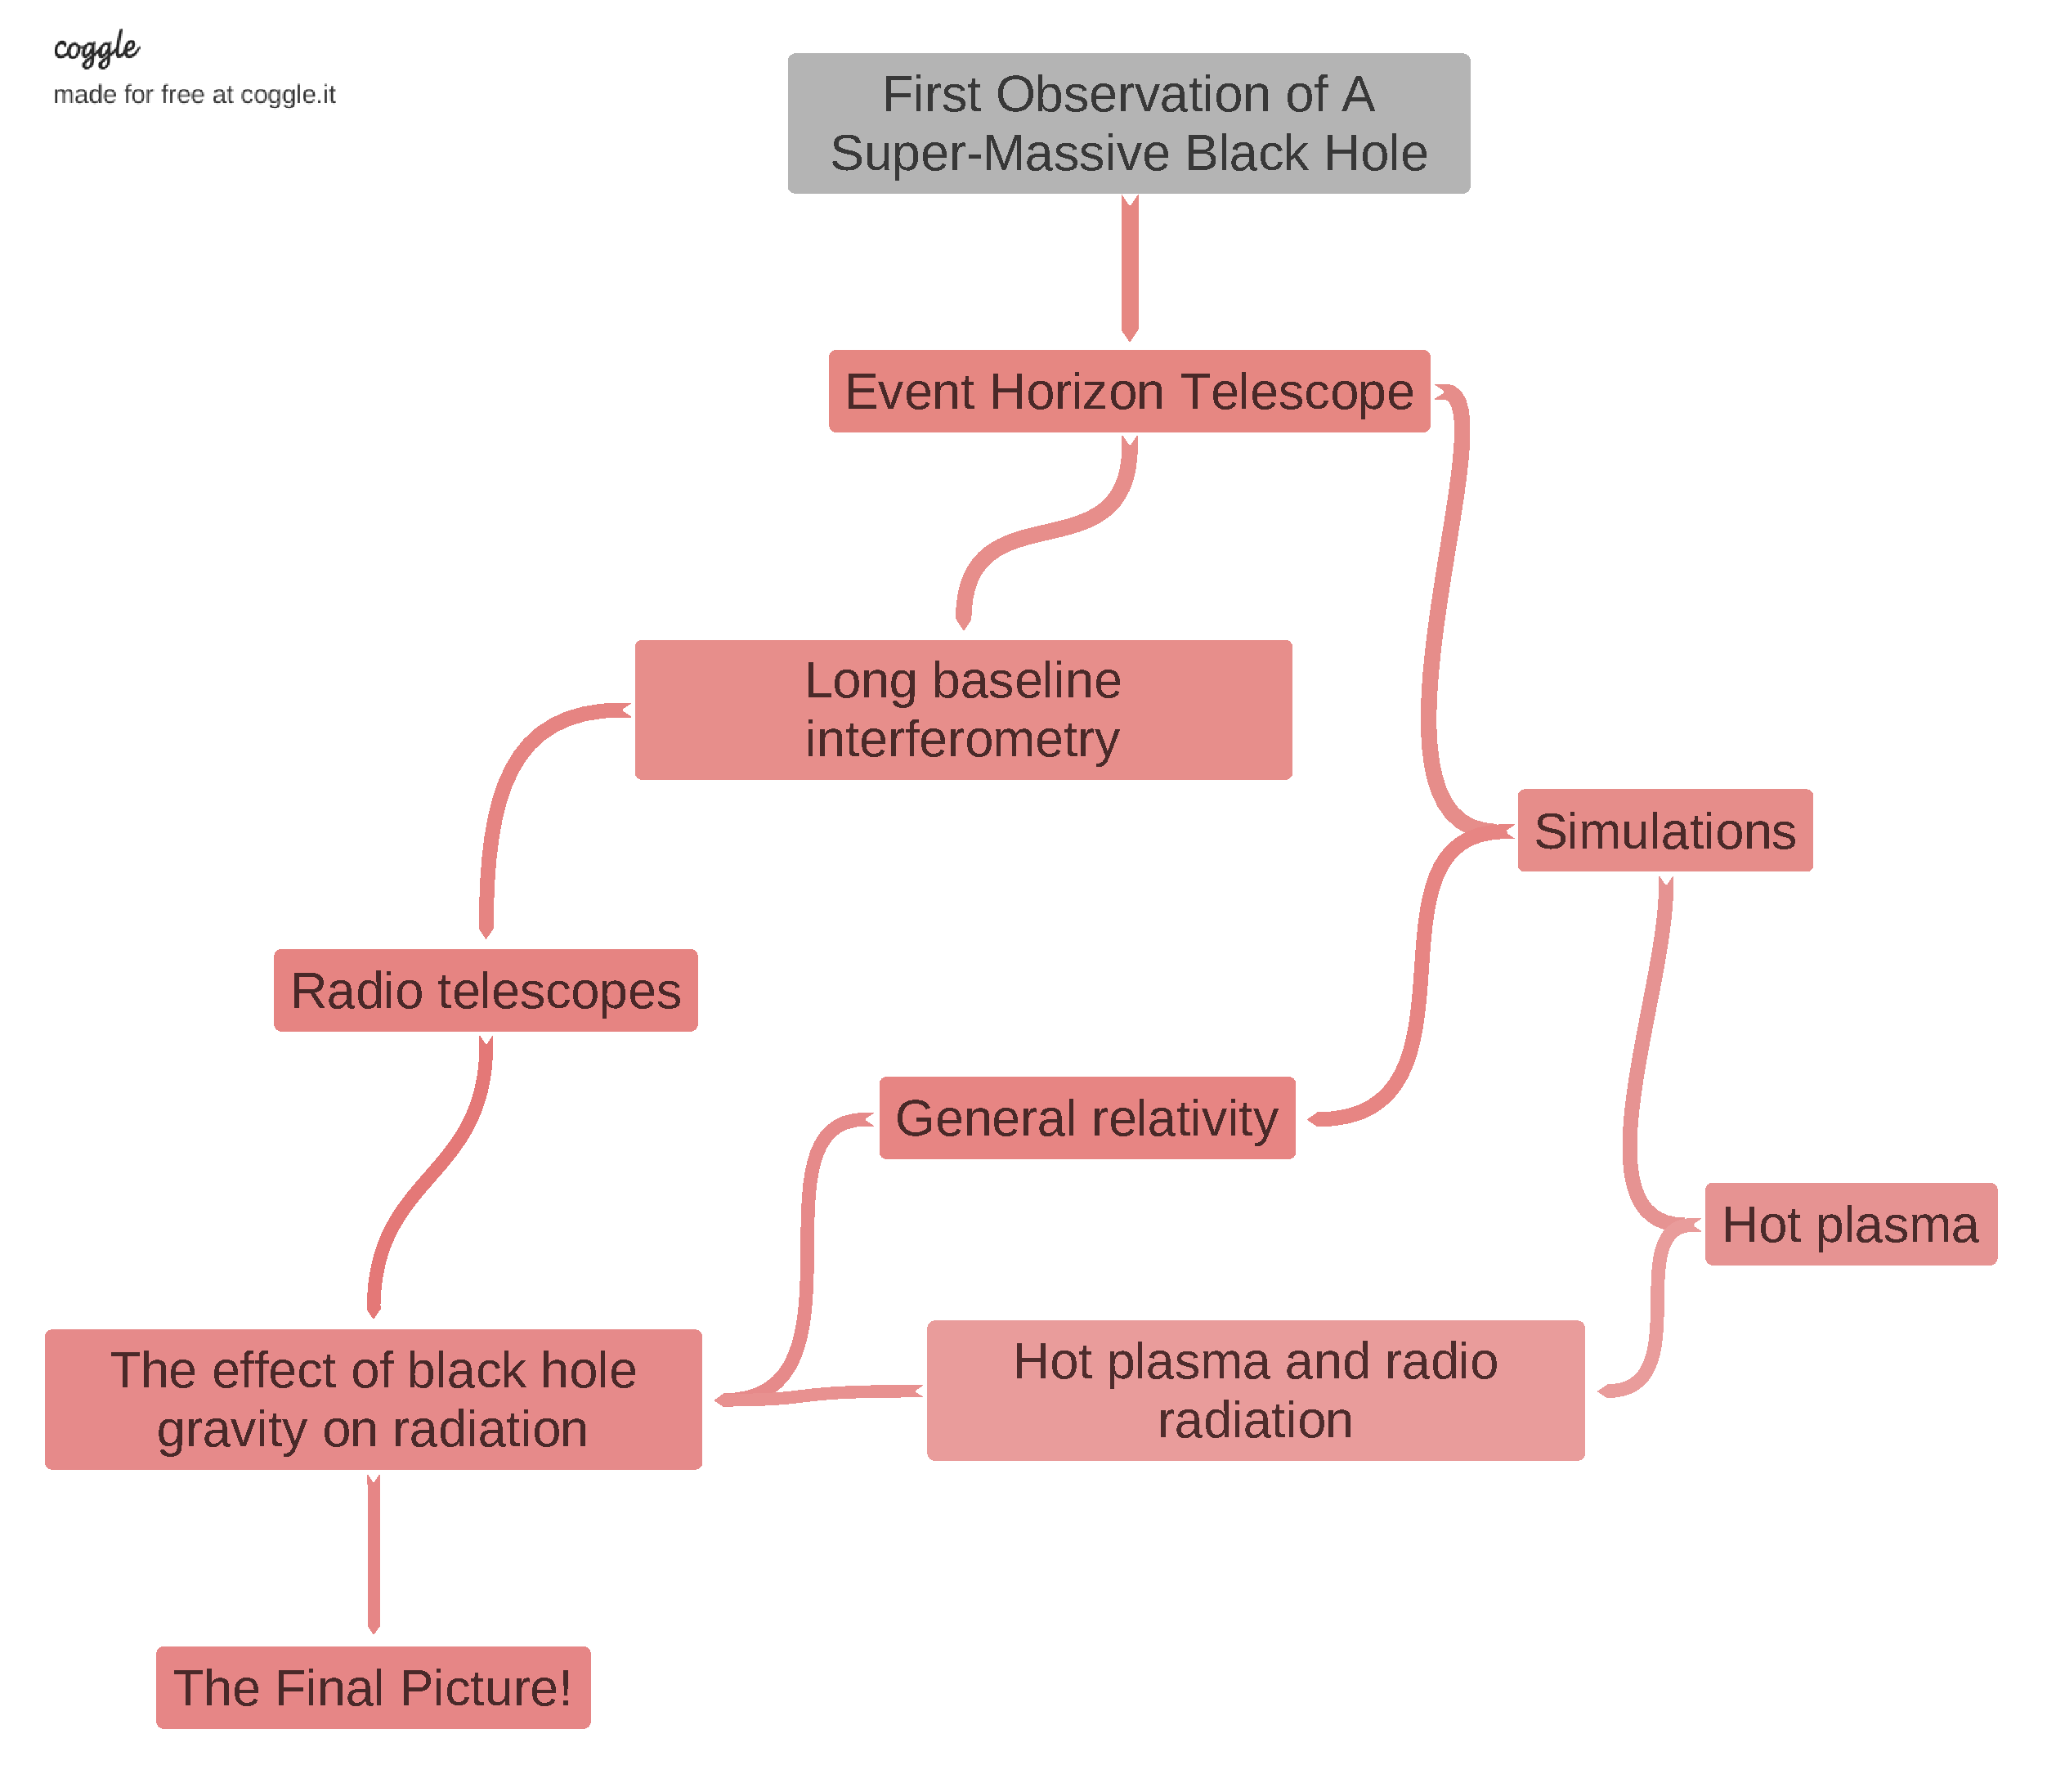
\includegraphics[width=0.65\textwidth]{figures/blackhole2.pdf}
\caption{\label{fig:black2} Black hole observations and Event Horizon Telescope, take 2.}
\end{figure}
\end{frame}

\section{Example: COVID-19 for a General Audience}

\begin{frame}{COVID-19 for a General Audience}
Review of general steps:
\begin{itemize}
\item Build a small list of sources
\item Create a map or outline
\item Write for each bubble or branch
\item Edit and polish the finished tract
\end{itemize}
\end{frame}

\begin{frame}{COVID-19 for a General Audience}
\alert{How do you ... \textit{start} ... building a set of sources?}  The first one is a \textit{general article} (written very well, sourced by a credible expert) for a general audience with links to technical work.
\begin{enumerate}
\item ``5 things scientists know about COVID-19 - and 5 they're still figuring out.'' Karen Frances Eng for \url{ideas.ted.com}
\item ``Tracking the Cornonavirus in California.'' LA Times
\item \url{https://coronavirus.jhu.edu/map.html}
\item \url{https://ourworldindata.org/coronavirus-data-explorer}
\end{enumerate}
\end{frame}

\begin{frame}{COVID-19 for a General Audience}
\begin{figure}
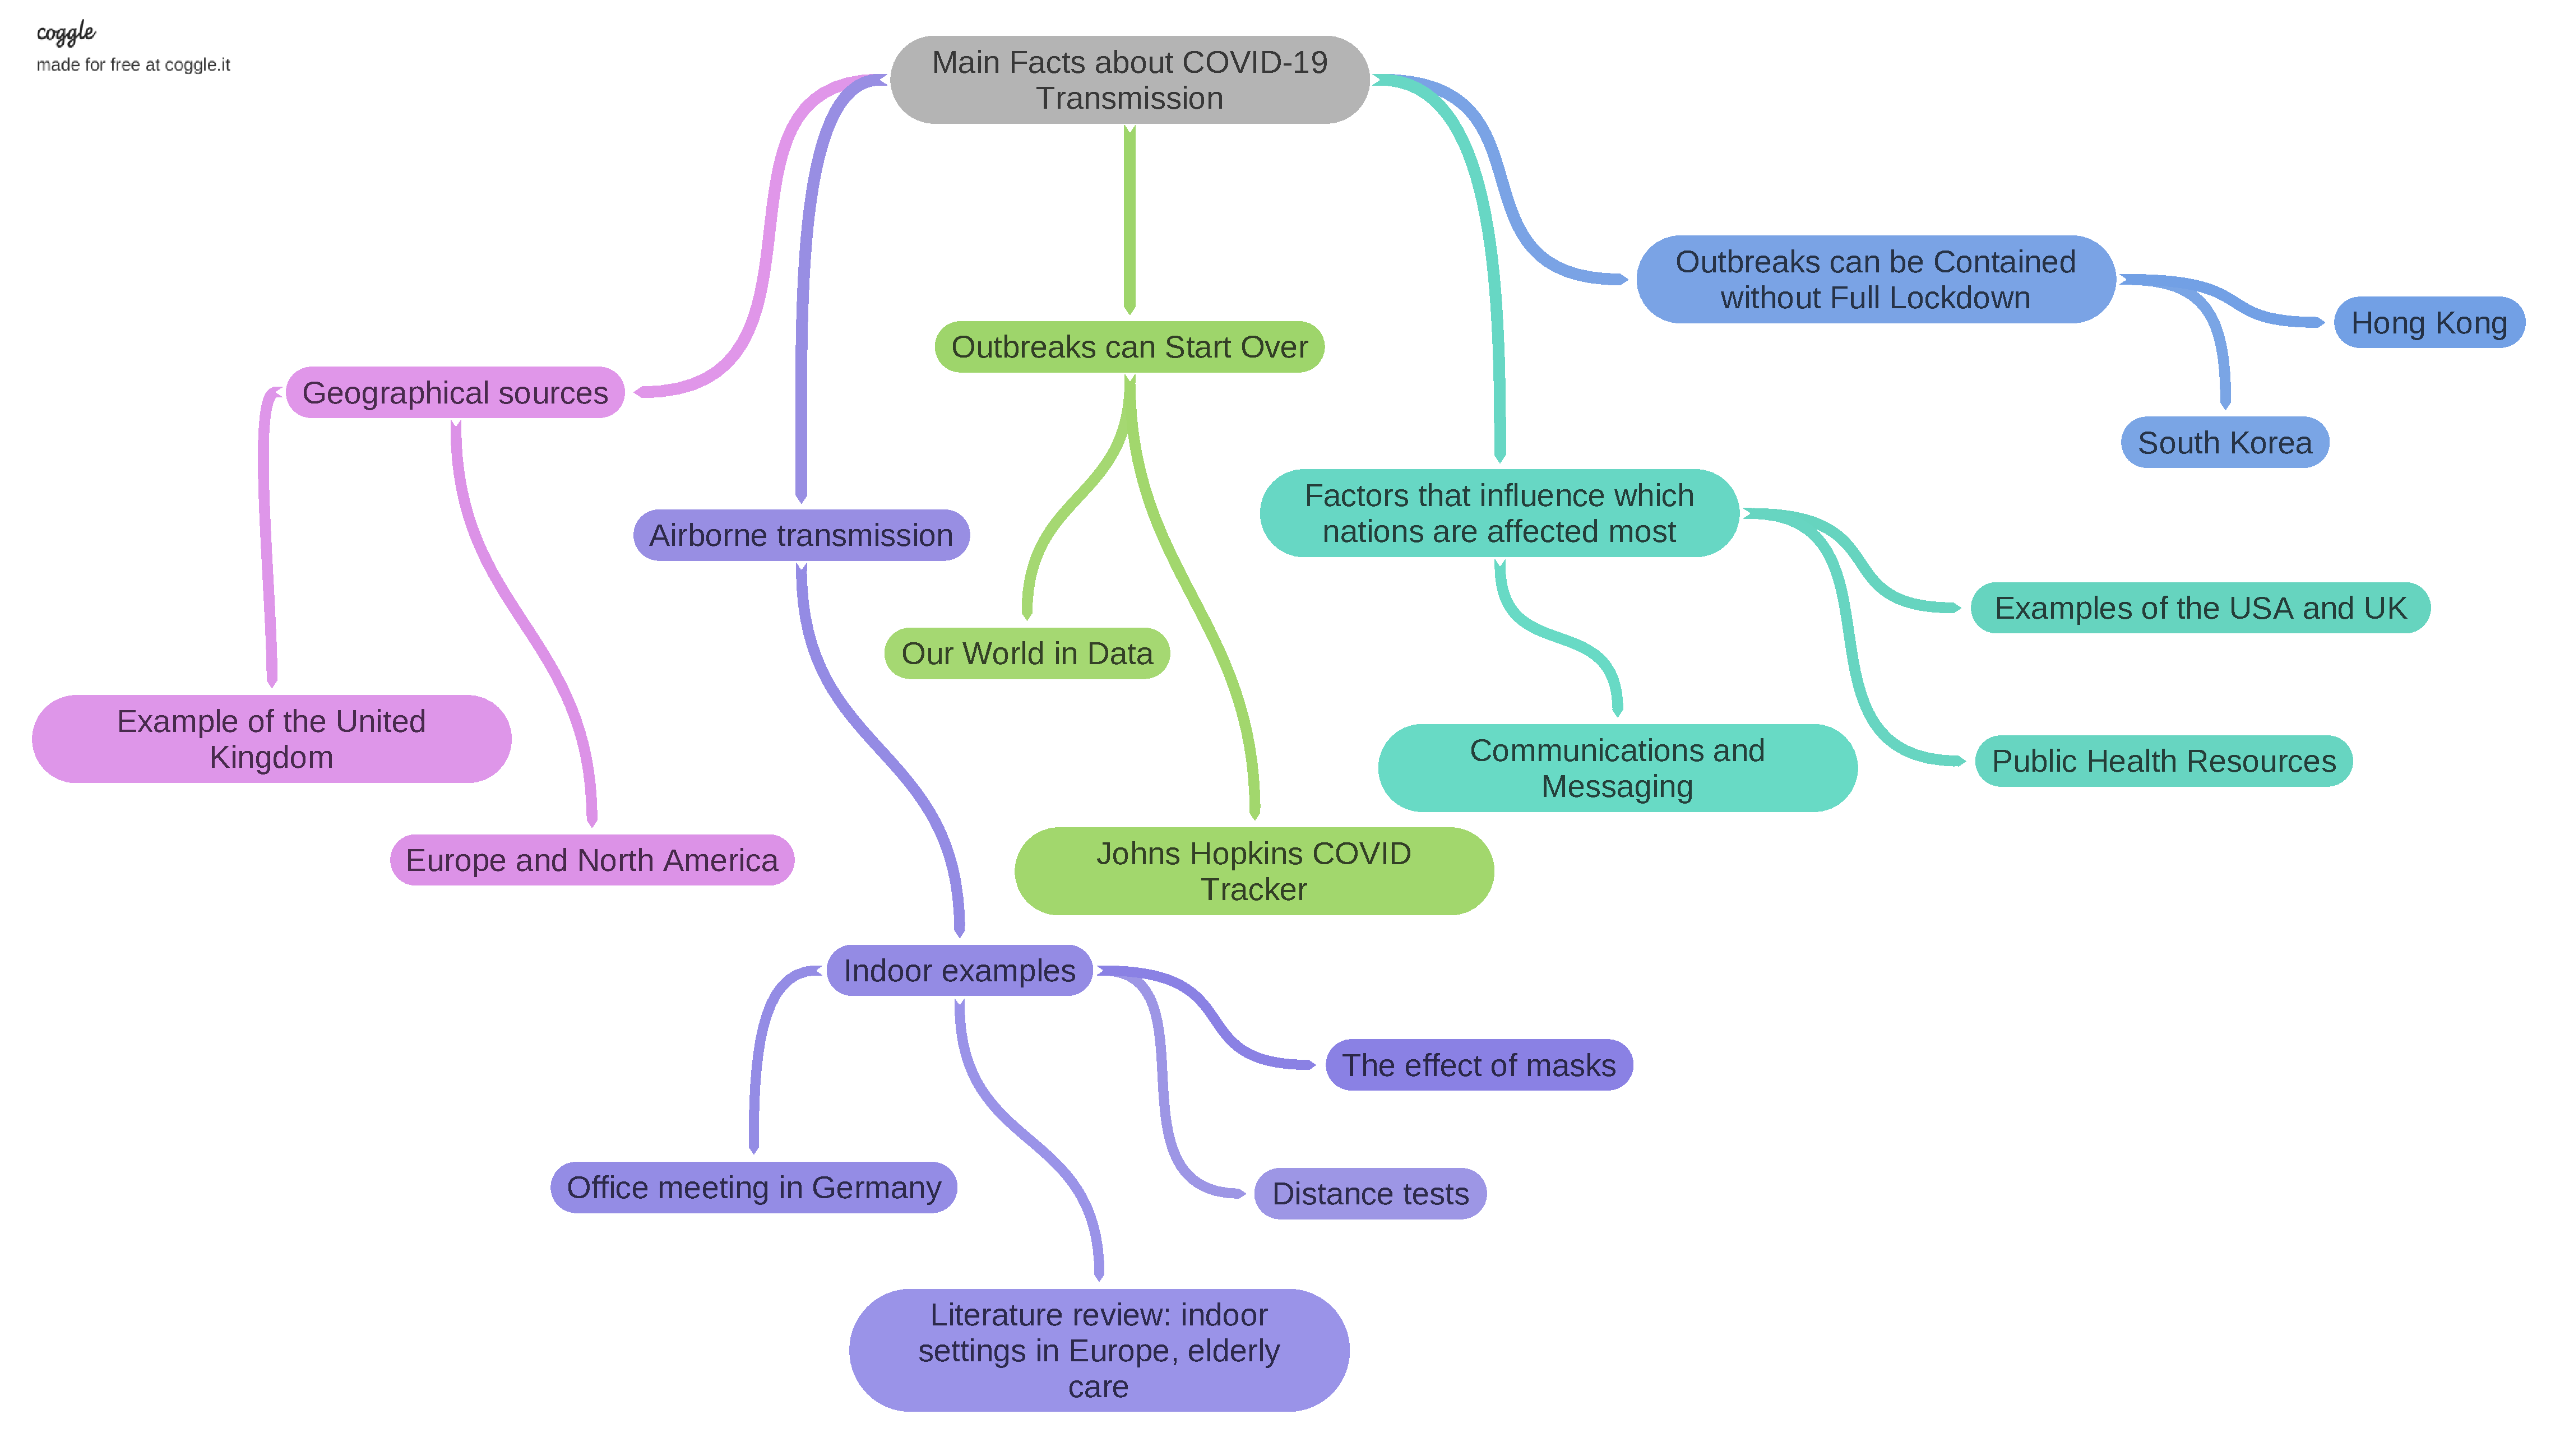
\includegraphics[width=0.95\textwidth]{figures/COVID_map.pdf}
\caption{\label{fig:covid1} This is an example of a mind map of the 5 things article.}
\end{figure}
\end{frame}

\begin{frame}{COVID-19 for a General Audience}
This could be a basic strategy in this extended example:
\begin{enumerate}
\item Start with the 5 things article
\item Branch off to the technical work
\begin{itemize}
\item What is research, and what is basic public health information
\item What is \textit{peer-reviewed} versus non-peer-reviewed work
\end{itemize}
\item Decide how much detail to keep from each branch
\item Interpret the graphs and the numbers: a few tips
\begin{itemize}
\item Never neglect the axes, always...\textbf{ALWAYS} define the axes for the reader
\item When describing shapes or curves or points on a chart, always use precise language
\item Avoid vague adjectives
\end{itemize}
\item Polish: use the delete button, use metaphor where appropriate, keep details in a hierarchy
\end{enumerate}
\end{frame}

\begin{frame}{COVID-19 for a General Audience}
\begin{figure}
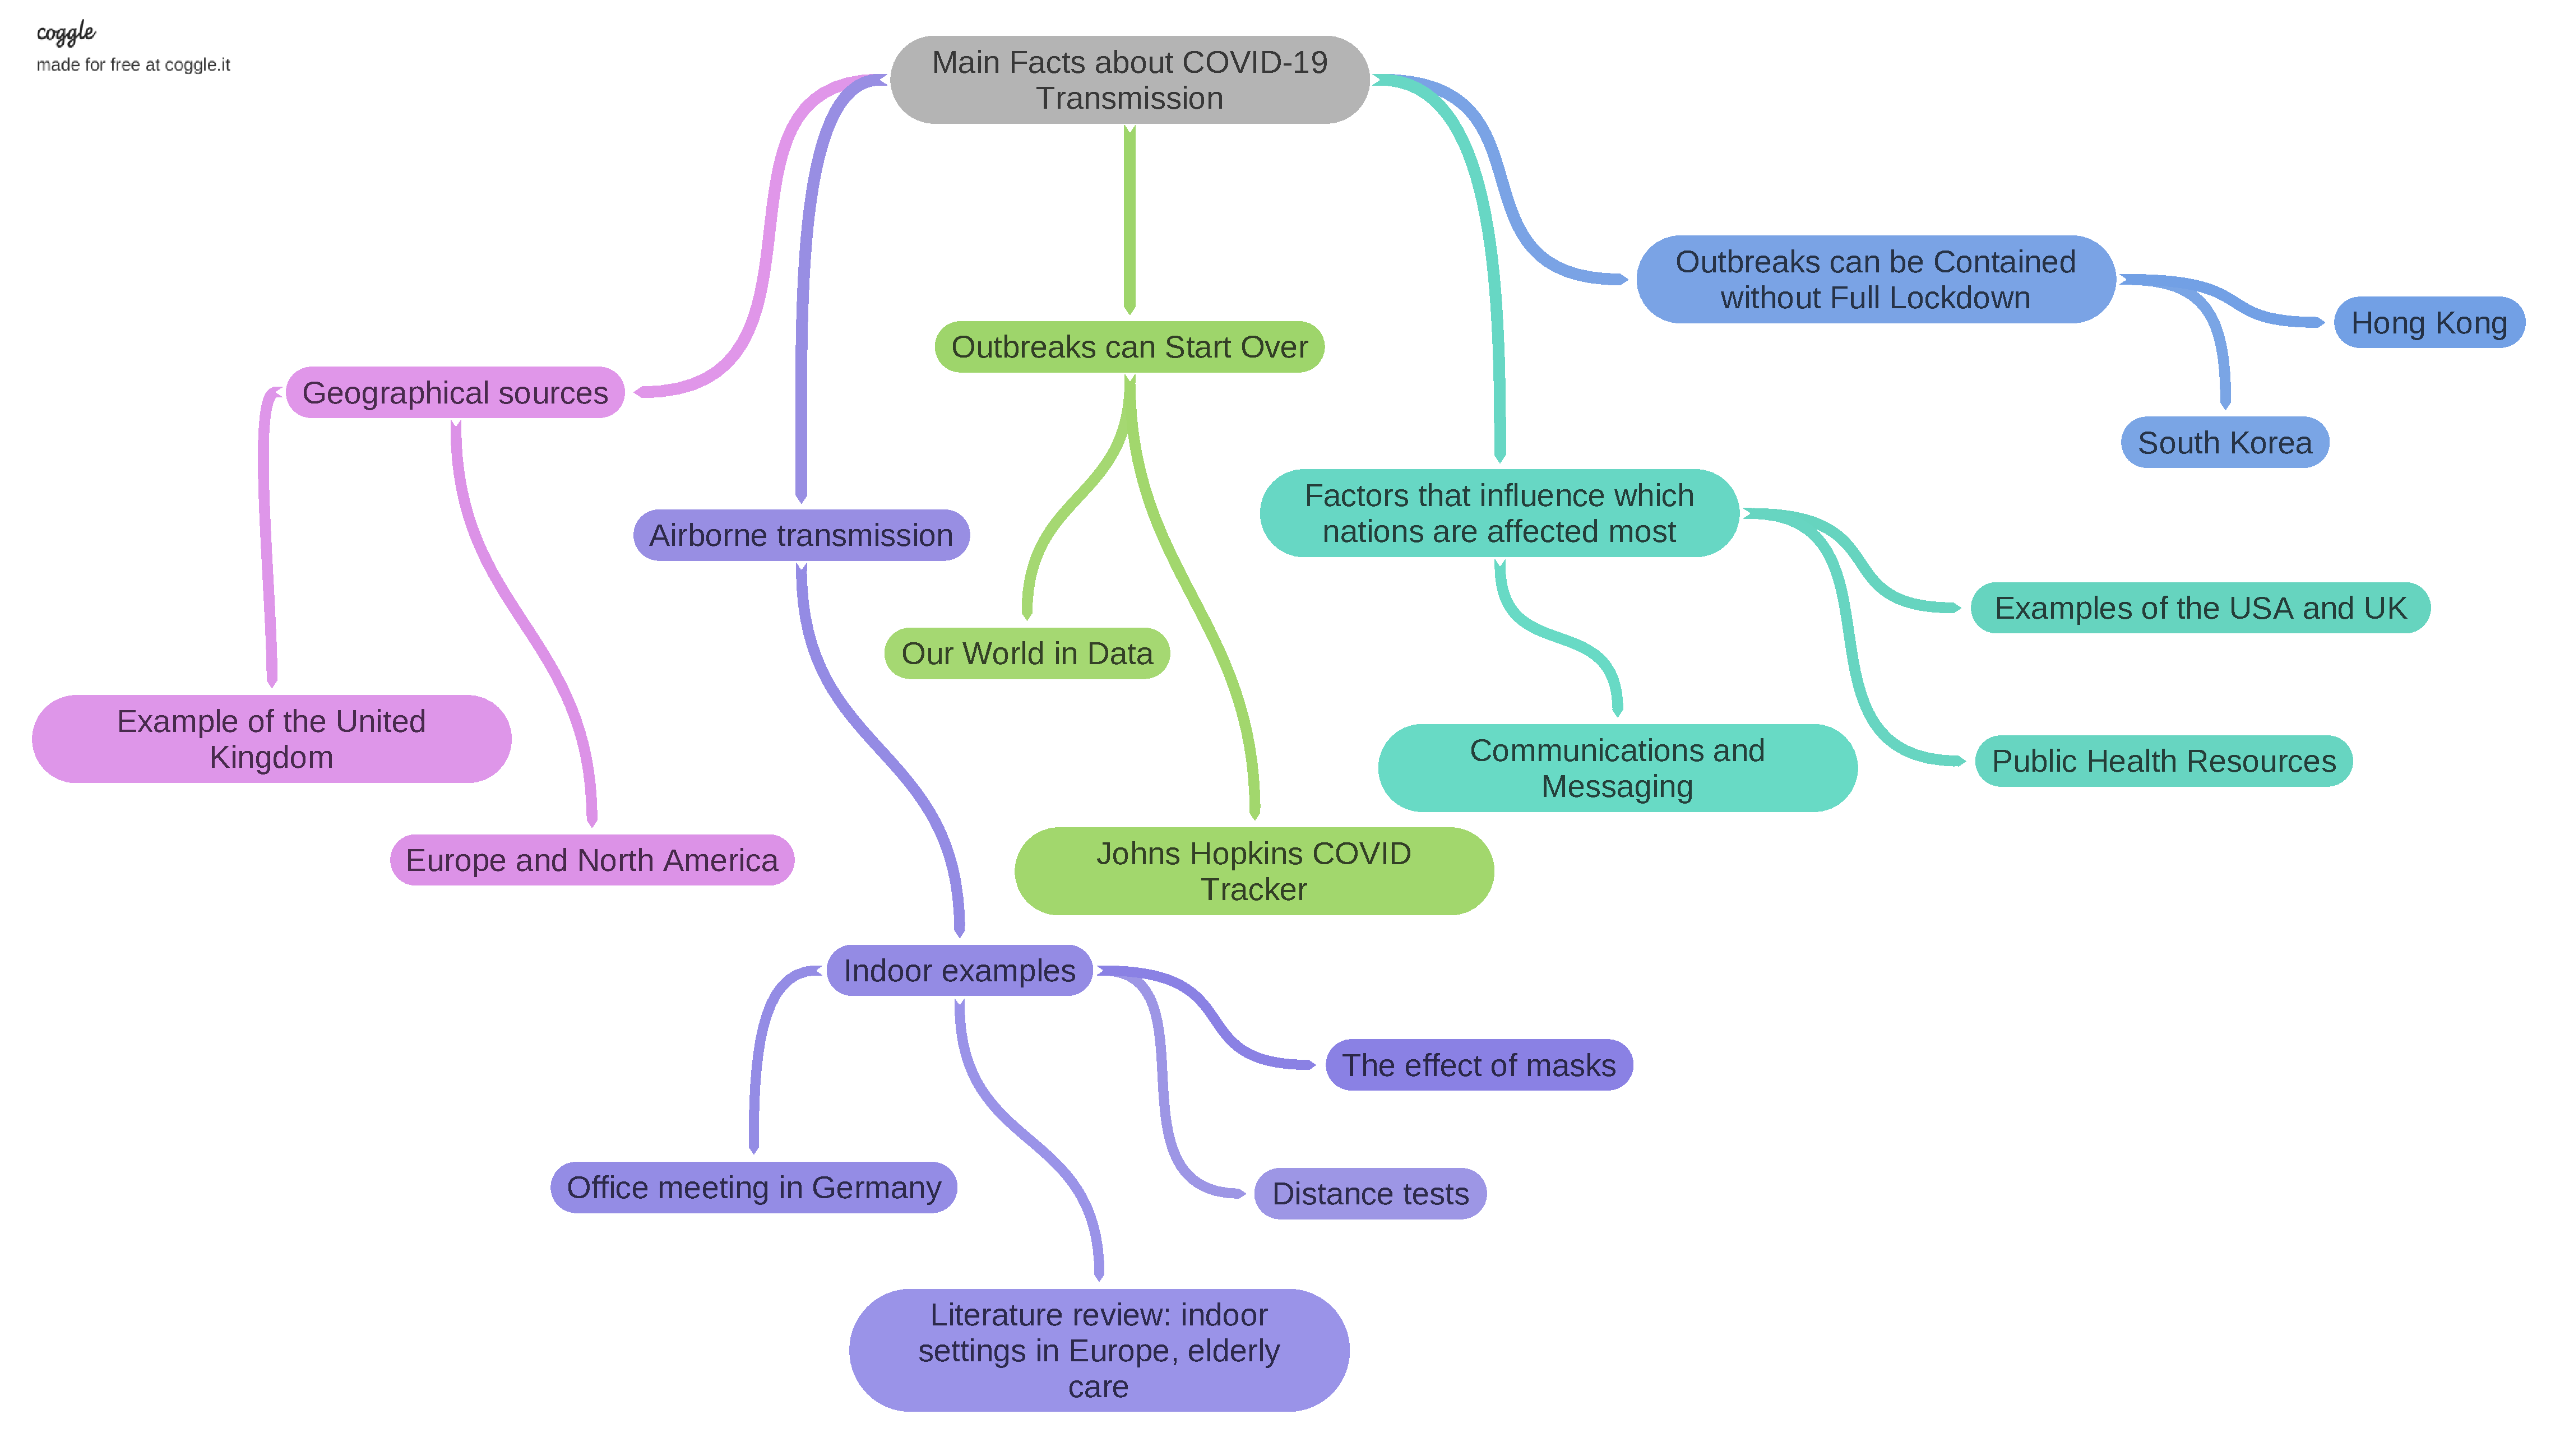
\includegraphics[width=0.95\textwidth]{figures/COVID_map.pdf}
\caption{\label{fig:covid2} This is an example of a mind map of the 5 things article.}
\end{figure}
\end{frame}

\begin{frame}{COVID-19 for a General Audience}
\textbf{Collaborate on Google Docs}: Go to Google Docs and log in with your Whittier College credentials.  Click on Shared with Me, and you should see the agenda page for today entitled Concise Writing, 2.  Using the Coggle map I've created, let's start writing!
\begin{enumerate}
\item Group A: Pink branch
\item Group B: Purple branch
\item Group C: Teal branch
\item Group D: Blue branch
\item Dr. Hanson: Lime branch
\end{enumerate}
Aaaaand...go!
\end{frame}

\section{Conclusion}

\begin{frame}{Summary}
\textbf{Week 2}: \textit{Concise writing II:} In Week 2, we will focus on reading a piece of science writing, and creating your \textit{own} writing that tailors the story to a particular audience.
\begin{itemize}
\item Exercises: work in teams to produce a piece of science writing intended for a broad audience that weaves together information from a variety of sources: (a) a TED talk (b) a scientific journal article (c) and resources like Wikipedia and Google Scholar
\item Homework: writing a post designed for social media about a piece of science that grabs the attention of a wide audience, and attempts to convince that audience that the science is interesting
\item Exploration topic: Black hole observations
\end{itemize}
\end{frame}

\bibliographystyle{plain}
\section{Bibliography}

\bibliography{bibfile}

\end{document}
